\documentclass[12pt,fleqn]{article}\usepackage{../common}
\begin{document}
Ders 10

Bugunku konumuz kritik noktalarin minima mi, maksima mi, yoksa eger noktasi
mi oldugunu anlama teknikleri. Kritik noktalar kismi turevlerin hepsinin
sifir oldugu noktadir, mesela 2 degiskenli fonksiyon icin $f_x=0$, $f_y=0$
olmalidir. 

3 degisik kritik nokta cesidi gorduk, lokal minima, lokal maksima, ve
eger (saddle) noktalari. 

Bir fonksiyonun birden fazla kritik noktasi olabilir. Mesela soyle bir
fonksiyon

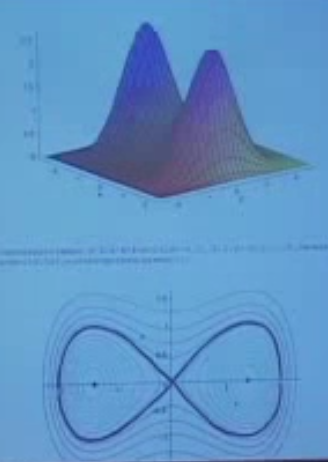
\includegraphics[height=4cm]{10_1.png}

Soru: Bir kritik noktaya bakarken, hangi kategoriye ait oldugunu nasil
anlayacagiz? Bir diger soru, global (lokal olmayan) minimum ve maksimum
noktalarini nasil buluruz?  Ustteki resimdeki fonksiyonda iki lokal
maksimum var. Her ikisini de deneyebiliriz, hangisi daha yuksek ise onu
aliriz. Diger yandan, bu fonksiyonun minimumu herhangi bir ``noktada'' degil,
maksimumdan uzakta, fonksiyonun en dis yerlerinde, sonsuzlukta. 

Yani global minimum ve maksimum illa bir noktada olmayabilir, sonsuzlukta
olabilir, o zaman bu kosulu test etmeliyiz, fonksiyonumuzun sonsuzluga
giderken nasil davrandigini anlamaliyiz.

Birinci soruyu cevaplayalim

Ikinci Turev Testi

$w = ax^2 + bxy + cy^2$

Bu fonksiyonun kritik noktasi orijinde. Eger turevleri alirsak, ve sifira
esitlersek, sonuc $x,y=0$ cikar. Ayni sekilde eger $w$'nin lineer
yaklasiksallamasini yapsaydik esitlik sagindaki butun terimlerin $x,y$
kucuk iken $x,y$'den kucuk oldugunu goruruz, o zaman grafigin tegeti $w=0$
noktasindadir. Eger orijinden ufak bir adim atarsak, o adimlarin fonksiyon
uzerindeki etkisi kare alma operasyonu yuzunden daha kuculur ($0.001^2 =
0.00001$ 
mesela). Herhangi bir noktadaki egim fonksiyon / degiskenlerdeki artis
olduguna gore, orijine yakin olan egim yukari dogru neredeyse yok gibidir. 

Ornek

\[ w = x^2 + 2xy + 3y^2 \]

Ustteki formulu su sekilde donusturursek

\[ w = (x+y)^2 + 2y^2 \]

Ustte iki karenin toplami var, karelerin ikisi de negatif olamaz, o zaman
minimum'un orijin olmasi gerekir (negatiflesmeden olabilecek en kucuk deger
oradadir). 

Birazdan gorecegiz ki ustteki kare tamamlama (completing the square)
yontemini $a,b,c$ katsayilarini iceren genel durum icin de kullanabiliriz. 

Once $a \ne 0$ farz etmem lazim, yoksa teknigin geri kalani mumkun olmaz. 

\[ w = a \bigg( x^2 + \frac{b}{a} xy \bigg) + cy^2 \]

Eger bir kare denklemin orta teriminde $b/a \ xy$ (ustteki gibi) elde etmek
istiyorsam, kare icinde $x$ ve $b/2a \ y$ terimlerini kullanirim, cunku bu iki
terimin birbirleri ile carpilip iki kere toplanmalari $b/a \ xy$ sonucunu
verir. O zaman

\[ = a \bigg( x + \frac{b}{2a}y  \bigg)^2  + ... \]

Hala isimiz bitmedi, kare icine koyulan $y$ yuzunden ortaya cikan $y^2$ bazli
terimi dengelemek gerekiyor,

\[ = a \bigg( x + \frac{b}{2a}y  \bigg)^2  + 
\bigg( c - \frac{b^2}{4a} \bigg)y^2
 \]


\[ = \frac{1}{4a} 
\bigg[
4a^2 \bigg( x+\frac{b}{2a}y \bigg)^2 +
\bigg(4ac - b^2 \bigg)y^2
\bigg]
\]


Bu noktada kontrol etmemiz gereken 3 durum var:

1) $4ac - b^2 < 0 => $ Ustteki ikinci terim negatif, pozitif $y^2$'yi
carpiyor yani negatiflik daha da buyuyor, birinci terim kesinlikle pozitif
(cunku karesi alinmis ifadeler var). Bu durumda bir eger noktamiz var. 

2)  $4ac - b^2 = 0 => $ Ikinci terim yokolur. Geri kalanlar sonucunda
fonksiyonumuz sadece bir yonde tanimli hale gelir, fonksiyonun ``dejenere''
oldugu soylenir. Mesela $w = x^2$ fonksiyonu boyledir, $y$'ye hic baglanti
yoktur, alttaki gibi.

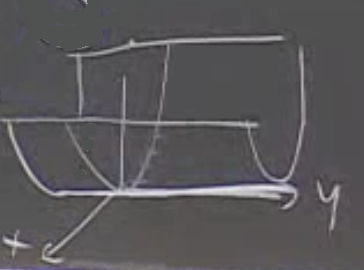
\includegraphics[height=3cm]{10_2.png}

Grafikte goruldugu gibi $y$ yonunde hicbir degisim olmamaktadir, o yonde
pek cok kritik nokta vardir, bu noktalar ``dejeneredir''. 

Ana formulumuzdeki birinci terimde $x$ ve $y$ olmasi sasirtici gelebilir,
orada $x$ ve $y$ oldugu icin elimizde dejenere bir durum var, eger o
ifadeleri kullanarak yeni bir eksen sistemi yaratsaydim, o yonde hicbir
degisiklik olmadigini gorurdum.

3) $4ac - b^2 > 0 => $ Bu durumda ustteki formulde, kareli ifadeler 

\[w = \frac{1}{4a} 
\bigg[
+ .. \bigg( .. \bigg)^2 +
\bigg( .. \bigg)
\bigg]
\]

hep $>0$ demektir, bu durumda elimizde ya bir maksimum ya da bir minimum
var. Isler $a$'ya gore degisecek, o zaman onun isaretine bakariz. 

Eger $a > 0$ bir minimum vardir

Eger $a < 0$ bir maksimum vardir

[bazi bolumler atlandi]

Genel olarak maks, min islemleri icin 2. turevlere bakmak gerekir. 

Kac turlu kismi turev vardir? Mesela bir kez $x$'e gore kismi turev alabilirim,
sonra elde ettigim fonksiyonun bir daha $x$'e gore turevini alirim. 

\[ \frac{\partial f^2}{\partial x^2} = f_{xx}\]

Ya da

\[ 
\frac{\partial f^2}{\partial x \partial y} = f_{xy}
 \]

Ya da 

\[ 
\frac{\partial f^2}{\partial y \partial x} = f_{yx}
 \]

Burada bir iyi haber su: Ustteki iki kismi turev birbirine esit, yani
$f_{xy} = f_{yx}$.

Ve en son olarak

\[ \frac{\partial f^2}{\partial y^2} = f_{yy}\]

2. Turev Testi

$f$'in kritik noktasi $x_0,y_o$'da $A = f_{xx}(x_o,y_o)$, $B =
f_{xy}(x_o,y_o)$, 
$C = f_{yy}(x_o,y_o)$ ise, o zaman 

\[ AC - B^2 > 0 \]

hesabina bakilir. Bu hesabin da 2 tane alt secenegi vardir. 

$A > 0$ ise lokal minimum. 

$A < 0$ ise lokal maksimum. 

\[ AC - B^2 < 0 \]

hesabi var ise, elimizde bir eger noktasi vardir. 

\[ AC - B^2 = 0 \]

ise hicbir sonuca varamayiz. Bir sekilde dejenere oldugunu biliriz, ama
nasil bir kritik nokta oldugunu bilemeyiz. 

Simdi formulumuz $w = ax^2 + bxy + cy^2$ uzerinde buldugumuz ozel sarti
kismi turevler ile dogrulayip dogrulayamayacagimiza bakalim. 

\[ w_{x} = 2ax + by\]

\[ w_{xx} = 2a\]

\[ w_{xy} = b\]

\[ w_{y} = bx + 2cy \]

\[ w_{yx} = b \]

O zaman

\[ A = 2a \]

\[ B = b \]

\[ C = 2c \]

\[ AC - B^2 = 4ac - b^2 \]

Gordugumuz gibi $4ac - b^2$ tekrar elde ettik, yani ilk basta kare
tamamlayarak elde ettigimiz irdelemeleri aynen kullanabiliriz. 

Tabii dejenere konumda hala ne yapilacagini bilmiyoruz. O durum icin de
Taylor Yaklasiksallamasini kullanacagiz. 

Karesel yaklasiksallama

\[ \Delta f \approx f_x (x - x_0) + f_y (y - y_0) \]

Fakat kritik noktalarda $f_x = f_y = 0$ oldugunu hatirlarsak, o zaman
ustteki ifadede tum terimler iptal (sifir) olur. Bu isimize yaramaz. Daha
fazla terim eklememiz lazim. 

\[ \Delta f \approx f_x (x - x_0) + f_y (y - y_0)   \]
\[\hspace{1cm}  + 
\frac{1}{2}f_{xx}(x-x_0)^2 + f_{xy}(x-x_0)(y-y_0) + 
\frac{1}{2}f_{yy}(y-y_0)^2 \]

Bu durumda genel durum (case) karesel duruma indirgenmis olur. Ustteki
formulde 

\[ \Delta f \approx f_x (x - x_0) + f_y (y - y_0)   \]
\[\hspace{1cm} + 
\underbrace{\frac{1}{2}f_{xx}}_{1/2 A = a}(x-x_0)^2 + 
\underbrace{f_{xy}}_{B=b}(x-x_0)(y-y_0) + 
\underbrace{\frac{1}{2}f_{yy}}_{1/2 C = c}(y-y_0)^2 \]

kullanilabilir. 

Dejenere durumda ne olacagi daha yuksek turevlere baglidir. Biz bu dersti o
konuya girmeyecegiz. 

Fakat sunu soylemek gerekir ki 

\[ AC - B^2 = 0 \]

sartinin ortaya cikmasi, yani ``sonuca varamiyoruz'' noktasina gelmek
gercek hayatta pek olmuyor. 

Ornek

\[ f(x,y)= x + y + \frac{1}{xy}, \ \ x,y > 0 \]

Min, maks nedir? 

Kritik noktalari bulalim. 

\[ f_x = 1 - \frac{1}{x^2y} = 0\]

\[ f_y = 1 - \frac{1}{xy^2} = 0\]

\[ x^2y = 1 \]

\[ xy^2 = 1 \]

Ikinci formul birinciyi bolerse, 

\[ x/y = 1 \]

yer degistirince

\[ x = y => x = 1 \]

\[ y^3 = 1 => y = 1 \]

Tek kritik nokta $(1,1)$

Soru

Bu nokta 

\begin{enumerate}
   \item Lokal minimum
   \item Lokal maksimum
   \item Eger noktasi
   \item ???
\end{enumerate}

Cevaplayin. 

Cevap icin 2. kismi turevleri hesaplayalim. 

\[ f_{xx} = \frac{2}{x^3y} \]

\[  A = 2 \]
\[ f_{xy} = \frac{1}{x^2y^2} \]

\[ B = 1 \]

\[ f_{yy} = \frac{2}{xy^3} \]

\[ C = 2 \]

\[ AC - B^2 = 2 \cdot 2 - 1^2 = 3 > 0 \]

Demek ki bu ya bir lokal min, ya da lokal maks. 

\[ A > 0 \]

o zaman bu lokal min. Hatta bunun bir global min oldugunu da kontrol etmek
mumkun. 

Ya peki lokal maksimum? 

Maksimum herhangi bir kritik noktada degil, maksimum sonsuzlukta. 

$x \to \infty$, ya da $y \to \infty$, ya da $x,y \to 0$ iken, $f \to
\infty$. 

Genelde ustteki kontrolleri yapmak gerekir, neler oldugunu anlamak icin
once kritik noktalara bakilir, sonra sinirlarda (boundaries) neler olduguna
bakilir.


\end{document}
